\section{Basic Concepts}
\label{sec:Basic-Concepts}

EXIP is a C library written in a portable manner that implements the EXI format for
XML representation. Probably a better way of describing what is EXIP is to say what it is \emph{not}.
EXIP is not a tool for converting text XML documents to EXI and vice versa. Why is that then?
To start with, the XML to EXI conversion requires a XML parser that process the XML input.
The XML parser itself is at least as big chunk of code as it is the EXI parser and having them
both at the same time might not be
possible or desired on a resource constrained embedded system. Second, parsing
the text XML and then converting it to EXI effectively removes all the processing benefits of EXI.
Having said that, it does not mean that it is not possible to use EXIP in such scenario. For example,
it is planned as a future work to include a module in EXIP that performs exactly that: generating
corresponding EXI streams from a text XML input and vice versa. It is therefore an optional
behavior and not an only possible way of using the library. It is not even difficult to implement
such a module and the reader could do that as a practical exercise after going through this guide.

As a result of this design choice, EXIP cannot use (at least for now) the XML Schema format directly
to perform schema-enabled processing. This might sound as a big flaw in the implementation but is
just the opposite. XML Schema documents are plain XML documents and as such they have analogous EXI
representation. Working with the EXI representation of the XML Schema definitions brings all the
performance benefits of the EXI itself - faster processing and more compact representation.
Now, using static systems where the schema information is only processed at design time would
not make much difference. However, once you are faced with more dynamic systems that are
capable of handling schema information at run-time, the use of EXI representation is more
beneficial especially in networked embedded environments.

Yet another \emph{not} - EXIP is not compliant with DOM, SAX or StAX Application Programming Interfaces (APIs)
for XML processing. The single reason for that is the efficiency trade-off. All these APIs are
using string representation of the primitive data types defined by the XML Schema specification
such as float, integer, date etc. This means that when schema definitions are available these
types must be converted from native types to string and then back from string to native representation
in order to fit in the API. Once again this does not mean that you cannot use EXIP with applications
that require DOM, SAX or StAX interface. The EXIP API is low level and typed and requires a
wrapper module in order to provide the aforementioned interfaces, which again is scheduled for future work.

\begin{figure}[h!]
 \begin{center}
 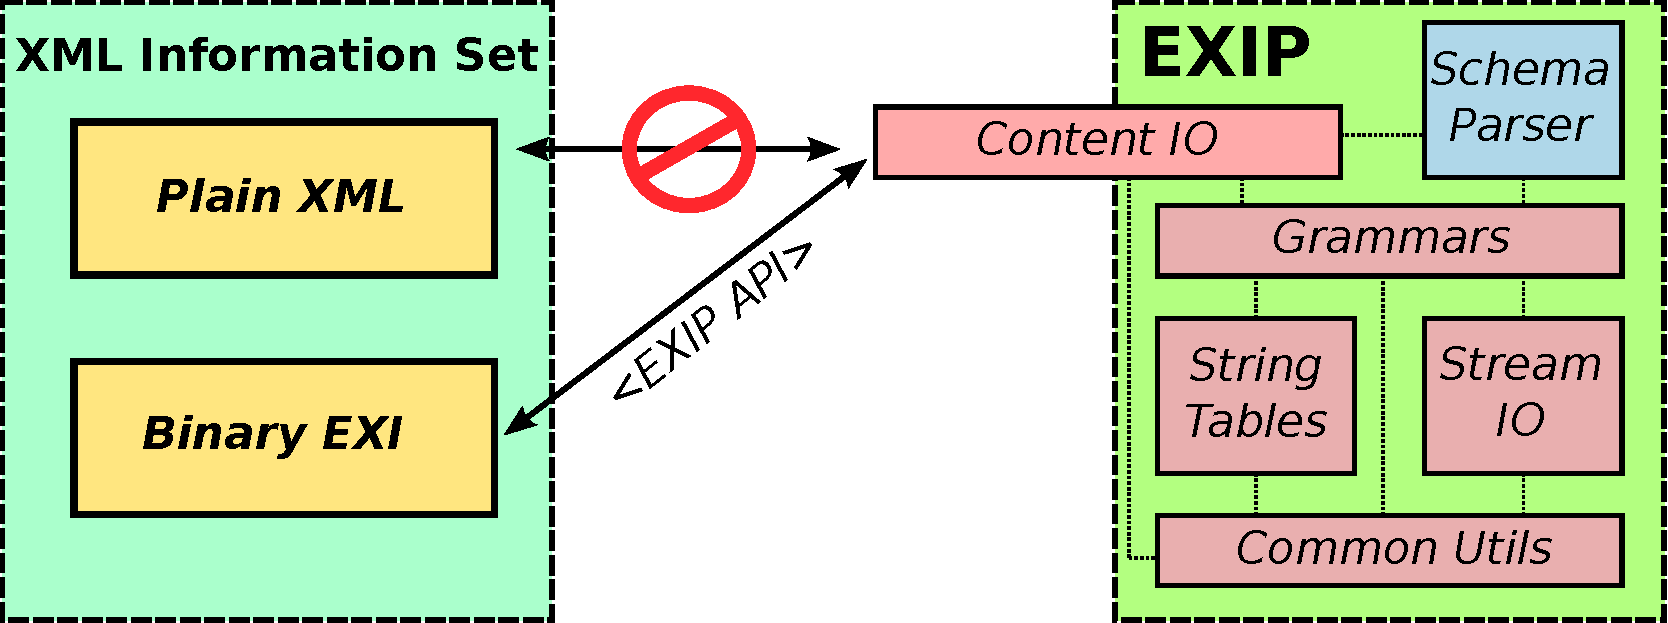
\includegraphics[width=0.90\textwidth, keepaspectratio=true]{images/EXIP-overview.pdf}
\end{center}
\caption{EXIP components}
\label{fig:EXIP-components} 
\end{figure} 

Figure \ref{fig:EXIP-components} depicts these design decisions and shows the different components of
the library. Key concept when creating the structure of the project was modularity - the functionality
is grouped and encapsulated in different components. This allows for disabling features that are not
needed directly at compile time. As an example, the Schema Parser component that is responsible for
generation the grammar structures based on XML Schema definitions is only needed if the system is
expected to dynamically handle XML schemes and hence in all other cases can be removed from the build at compile time. 

For further information and details on the EXIP API and the rational
behind it see the paper that first presents EXIP \cite{RumenKyusakov2011} (please refer to this work when 
citing information from this guide or other EXIP documentation).

\subsection{Project structure}
\label{sec:project-structure}

The EXIP library is an Eclipse C project (and MS Visual Studio 2010 solution)
structured in the following subdirectories:
\begin{itemize}
 \item \texttt{bin/} - this is the build output directory. It is automatically created/removed when
doing builds of the project. The library binaries are located directly into the \texttt{bin/} folder
while the examples and other utils are compiled in separate subfolders

 \item \texttt{build/} - this folder contains the build scripts of the project. The current release
provides a MS VS 2010 build under \texttt{build/vs2010/} and \emph{GCC} toolchain builds under \texttt{build/gcc/}.
The \texttt{build/gcc/} folder further contains platform-dependent parameters and
headers located in subfolders - \texttt{build/gcc/mulle} for the Mulle sensor platform,
\texttt{build/gcc/oe-armv5te} for OpenEmbedded Linux on ARMv5te and the default
\texttt{build/gcc/pc} for descktop PCs. The build is started from \texttt{build/gcc/} with the following
\texttt{make} build targets available:
\begin{description}
 \item[all] compiles the EXIP library. The default target platform is PC. To change the target
platform to Mulle for example, add \texttt{target=mulle} as an argument of \texttt{make}
 \item[check] invokes the Check unit tests
 \item[clean] removes the \texttt{bin/} folder
 \item[doc] generates the project Doxygen documentation. The output directory is set to \texttt{doc/dev/doxygen/}
 \item[examples] compiles and builds the example executables
 \item[utils] compiles and builds the utils executables
 \item[lib] generates a static library libexip.a in \texttt{bin/lib}
 \item[dynlib] generates a dynamic library libexip.so in \texttt{bin/lib}
 \end{description}

 \item \texttt{doc/} - the project documentation: \texttt{doc/user/} contains the source of this user guide;
    \texttt{doc/dev/} is the development documentation; 
  \texttt{doc/www/} contains the information available on the project web page

 \item \texttt{examples/} - the root of the example applications shipped with EXIP

 \item \texttt{include/} - this folder contains the public header files of the EXIP library.
			  Together with the \texttt{exipConfig.h} defined per target platform, these files
			  define the public interface of the library.

 \item \texttt{src/} - here are all internal definitions and \texttt{.c} files divided into
	      subfolders according to the modules in which they belong

 \item \texttt{tests/} - Check unit tests, integration and validation tests

 \item \texttt{utils/} - supporting utilities and development tools

\end{itemize}


\subsection{Strings in EXIP}
\label{sec:strings}

All character strings in EXIP are length prefixed. This means that all the strings that are passed to
the EXI encoder and all the strings that are parsed from the decoder are in this format. The motivation
for that is the number of string comparisons that the EXI processor must perform when going through an
EXI stream. In many cases, when the strings differ in length, this operation is very efficient
when the length is saved together with the characters data. EXIP provides an API for working with
this type of strings defined in \texttt{stringManipulate.h}. The implementation of the functions
declared in this header file defines what type of characters are supported in the string.
For example, \texttt{ASCII\_stringManipulate.c} implements the strings as ASCII character arrays.

One way of increasing the compactness defined in the EXI specification is through the use of string tables.
The string tables are partitioned dictionary that stores and indexes the strings that occur in particular
EXI document. In such way, when a string has been used once in the document it is added to the string tables.
Every other occurrence of the same string in the document is represented by its index in the string tables.

\begin{figure}[h!]
 \begin{center}
 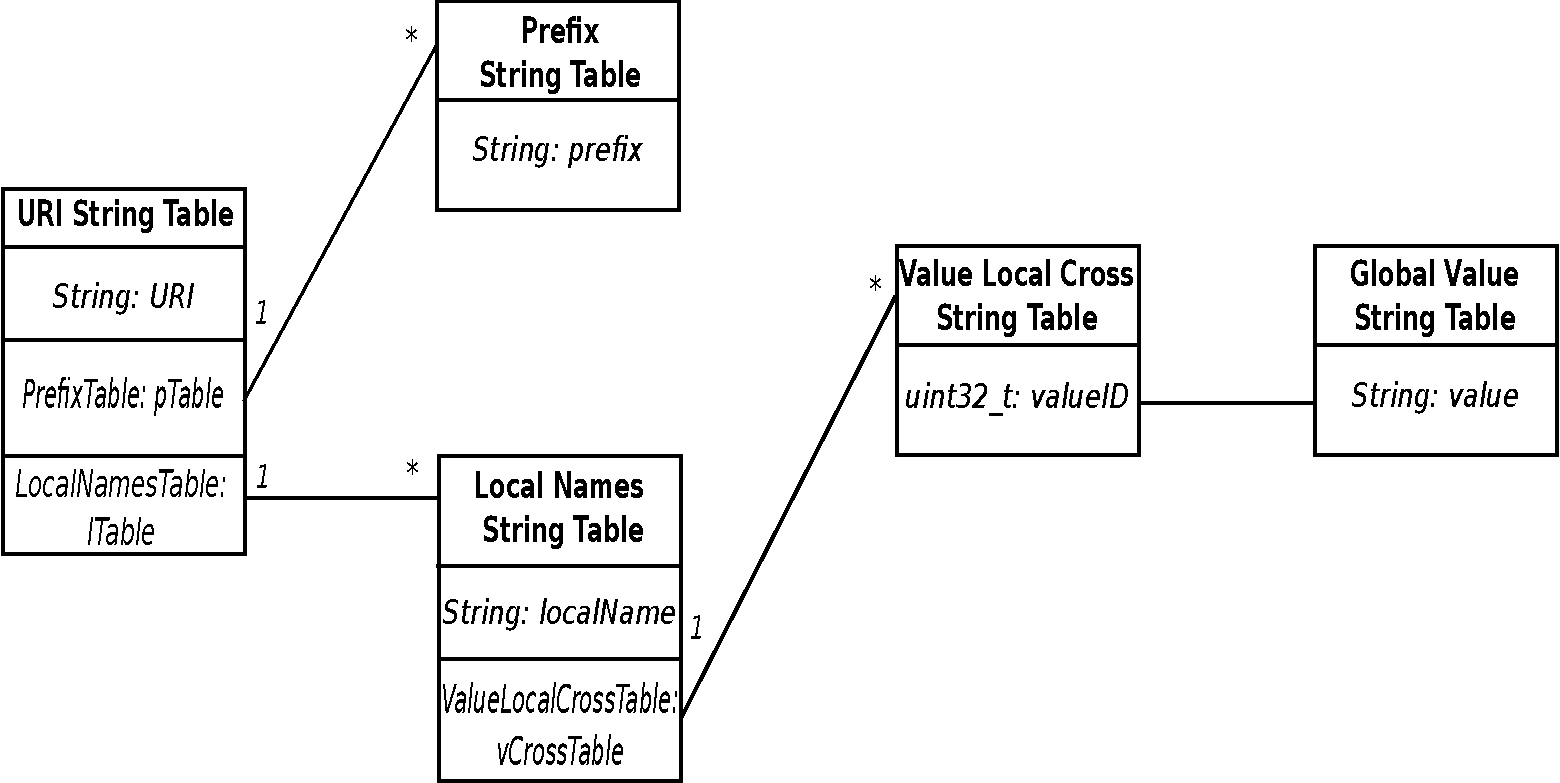
\includegraphics[width=0.90\textwidth, keepaspectratio=true]{images/StringTablesDiag.pdf}
\end{center}
\caption{String tables in EXIP}
\label{fig:EXIP-string-tables} 
\end{figure} 

Figure \ref{fig:EXIP-string-tables} shows how the string tables are implemented in EXIP. As a user of
the library you do not need to understand the actual implementation details. The only thing that you need
to be aware of is that the strings that are passed to your application by the EXIP parser should not be
modified as they are integral part of the string tables. You can clone the strings and use that copy
for string manipulations.

\subsection{Error handling and memory management}
\label{sec:errors-memory}
When an invalid input is given to the EXIP parser or some other error conditions occur, the
EXIP library functions return a numeric error codes that are defined in \texttt{errorHandle.h}.
More fine-grained error messages can be acquired by turning on the debugging routines.
You have control over the level of verbosity (INFO, WARNING or ERROR) and the source of
debugging information. All these parameters can be configured in the \texttt{exipConfig.h} header
that is defined per target platform in \texttt{build/gcc/<target\_platform>} or
\texttt{build/vs2010} for Windows.
When turned on the debugging information is by default printed on the standard output.

EXIP has an internal memory management infrastructure and you are not required to
know its details unless you are using the EXIP string type in your own applications. That is because
the string manipulation functions use \texttt{AllocList} to manage their allocations.
You can either define your own string manipulation functions or acquaint yourself with 
the memory management routines defined in \texttt{memManagement.h}.
